\documentclass[11pt]{article}
\usepackage{geometry}
 \geometry{
 a4paper,
 left=40mm,
 right=20mm,
 top=30mm,
 bottom=20mm,
 }
\usepackage[utf8]{inputenc}
\usepackage[english]{babel}
\usepackage[backend=biber, style=alphabetic]{biblatex}
\usepackage{amsmath, amssymb}
\usepackage{hyperref}
\usepackage{makeidx}
\usepackage{graphicx}

% For cryptography-related symbols (optional)
\usepackage{bbm}  % For blackboard bold symbols (e.g., mathbb{Z})
\usepackage{amsfonts} % For additional font styles

% Title
\title{YoDA network litepaper}
\author{YoDA Team}
\date{Draft - November 2024}
\addbibresource{references.bib}

% Begin Document
\begin{document}

\maketitle

\begin{abstract}
YoDA (Your own Data Availability) is a next-generation Data Availability (DA) solution powered by Instant Verifiable RAM (a low-latency DA network with instant finality and validity proofs). YoDA provides a cutting-edge, multi-layer technological stack that powers the seamless integration of different Web3 components without sacrificing usability or security. It combines DA with the Web2-level developer-friendly interfaces of familiar tools like Kafka, Redis, RabbitMQ, and S3, providing Web3 builders with the developer experience of traditional infrastructure. YoDA unlocks Layer 2 interoperability via trustless and secure cross-chain messaging protocol. It is powered by FRI commitments, achieving faster proving times than existing DA solutions based on KZG schemes. It leverages Byzantine fault tolerant (BFT) consensus with provable finality, allowing instantly finalized blocks with low latency, making it ideal for real-time, verifiable data interaction in decentralized environments.
\end{abstract}

\tableofcontents

\section{Introduction}
The rapidly evolving landscape of blockchain infrastructures and decentralized applications has created an urgent need for efficient, secure, and developer-friendly data availability solutions \cite{hasw:2023/1079}. Ethereum is moving towards a rollup-centric roadmap to enhance on-chain scalability, aiming to process hundreds of thousands of transactions through a decentralized, trustless “World Computer” \cite{inevitableeth}. In this framework, Ethereum Layer 1 (L1) acts as the settlement layer, confirming transactions and making them immutable. Rollups and app chains function as external coprocessors that enable fast execution while inheriting security from the L1. Finally, the memory allocation device is required to store the data to be processed, i.e. the RAM of the World Computer. This problem translates to blockchains as the storage of data related to transactions executed on Layer 2 (L2) must be made available on the L1 for future verification and confirmation. The problem of keeping this data in memory is not trivial and it is known today as the data availability (DA) problem \cite{hasw:2023/1079, AlBass18}. In particular, it is crucial to keep the transaction data available for on-chain verification; if the nodes cannot confirm the validity of a transaction then the entire system is exposed to incomplete verification of L2 transactions, hence potential fraud risks. 

Data availability sampling (DAS) \cite{hasw:2023/1079, AlBass18} promises to mitigate the DA problem. It is a cryptographic technique that allows the nodes of a network to verify data availability probabilistically by sampling small portions instead of downloading full blocks, thus enhancing validation efficiency. Ethereum plans to adopt DAS in the Danksharding upgrade \cite{eip4844, damato2023danksharding}. This update enables L2 rollups to post transaction data directly on the L1 without incurring in high fees. It is designed to scale Ethereum to handle hundreds of thousands of transactions per second while keeping costs manageable. However, Danksharding requires significant changes to the Ethereum protocol, including the introduction of a new block resource called ``blob data", the usage of polynomial commitments for blob verification, and the implementation of DAS at the consensus level. As a step toward Danksharding, Ethereum has been upgraded to Proto-Danksharding (EIP-4844) \cite{eip4844} first. This initial phase introduces blob spaces in blocks, a dedicated fee market, and the implementation of cryptographic structures to support DA validity proofs based on KZG commitments \cite{kzg-2010-23846}. While Proto-Danksharding has significantly reduced blob data costs, it remains inefficient because validators must download all data in its entirety. Consequently, Ethereum's blob space is currently limited to three blobs of approximately 125 kB per block, posing significant constraints for data-intensive use cases.
%
In contrast, projects like EigenDA, Celestia, and Avail \cite{eigenda, celestia24, avail24} store data blobs off-chain with the aim of improving both in accessibility and scalability. However, these solutions face different limitations. For example, Avail suffers slow DA confirmations and uses KZG commitments thus depending on a trusted setup; EigenDA entrusts a centralized component to encode and distribute blob data toward storage nodes, while Celestia combines Merkle tree commitments with fraud proofs that suffer of computation overheads and extra DA confirmation latencies. Overcoming these challenges is crucial for the large-scale adoption of the unified World Computer.

\smallskip

This litepaper introduces YoDA (Your Own Data Availability), a next-generation DA solution that provides efficient and secure data availability with an enhanced user experience. At its core is the innovative Instant Verifiable RAM (IVRAM), a low-latency and high-throughput DA component that offers instant finality and validity proofs for stored transaction data in a decentralized and permissionless manner. The IVRAM is a network of autonomous nodes that coordinate the generation and storage of submitted data blobs. It leverages a novel Byzantine Fault Tolerant (BFT) consensus protocol to ensure high performance and decentralization without incurring unwanted overheads. Each honest validator is responsible for verifying that data blobs are properly stored and available for final retrieval. The IVRAM ensures immediate accessibility and verifiable security, a crucial requirement for decentralized systems where trust and transparency are paramount.
%
YoDA provides secure and fast verification of data blobs by adopting cutting-edge cryptography based on FRI IOPPs \cite{bensasson18, hasw:2024/248}. At a high level, YoDA uses an FRI-based polynomial commitment scheme that efficiently generates commitments to the blob data with polylogarithmic verification times. Compared to other mainstream schemes like the KZG adopted by Proto-Danksharding and AvailDA, this approach offers several advantages: it inherently provides post-quantum security using hash functions, does not require a trusted setup, and enables faster proof generation.
%
On top of the IVRAM, YoDA offers unique services that promise to revolutionize Web3 application development and usability. The first service is the YoDA Interface Layer, which leverages the IVRAM to build efficient data engineering tools for high-demand applications. This layer introduces the concept of Decentralized Programmable Storage (DPS), providing the IVRAM with familiar interfaces like Kafka for stream processing, Redis for key-value storage, RabbitMQ for message queuing, and S3 for object storage. These tools allow developers to deploy their applications directly on the World Computer without needing external Web2 interfaces.
%
The second groundbreaking service is the YoDA Interoperability Layer. It allows interconnecting L2 systems like Rollups and Appchains with L1 blockchains like Ethereum and Solana. This layer facilitates smooth data transfer between systems without prohibitive waiting times for processing. For example, users can settle transactions on Ethereum while operating with data from an application deployed on Solana. Data stored on the IVRAM is instantly available across all interconnected components, enabling direct access to data and seamless integration between independent infrastructures.
%
The YoDA Interoperability and Interface layers utilize the IVRAM for efficient storage of data blobs with fast finality and high scalability guarantees. However, some use cases, like on-chain AI decision systems, may require pushing IVRAM performance boundaries toward quasi-instant DA. To this end, the YoDA Acceleration Layer allows fast DA pre-confirmations with an optimistic approach with almost zero latency.

\smallskip
YoDA lowers entry barriers for developers transitioning to decentralized systems by allowing them to use their existing knowledge and tools while benefiting from enhanced security and efficiency provided by YoDA.

\section{Problem Statement}
Despite advancements and widespread adoption of blockchain technologies, creating a World Computer capable of processing high volumes of transactions in a decentralized and efficient manner remains unachieved. Scalability and efficiency challenges must be addressed to achieve mass adoption.

\subsection{Data Availability Trilemma}
Existing DA layers face significant challenges, particularly in terms of high latency, slow finality times, and limited capacity. This is largely due to the Data Availability Trilemma that we introduce in this litepaper. This new trilemma states that a DA layer cannot achieve simultaneously:
\begin{itemize}
    \item \textbf{Security}: the probability that an attacker can manipulate or withhold data that has been made available. A secure DA solution should make it harder for an attacker to hide missing or compromised data.
    \item \textbf{Performance}: the ability to achieve low-latency and high-throughput DA confirmation, i.e., the expected time for blobs to be included in the DA layer and verified by clients.
    \item \textbf{Capacity}: the amount of bytes the DA layer can process per second; it relates to the number of blobs a DA layer submits per block. For example, Ethereum EIP-4844 allocates ~375 kB per block, such as three blobs of ~125 kB each, resulting in a capacity of ~31kB/s.
\end{itemize}

In figure \ref{fig:da-trilemma} we provide a visualization of the trilemma and how existing DA solutions position. The Ethereum Proto-Dankshard provides strong security and at the same time inherits slow-speed from the L1. Moreover, it cannot provide large capacity because propagating large blobs would be prohibitive at the Ethereum L1 scale. Other solutions like Celestia and Avail use off-chain validator networks to reach consensus and store data blobs on their ledgers with custom governance rules. Celestia finalizes blocks in 12 seconds using an optimistic approach that combines DAS with fraud proofs, leveraging a network of light clients that sample published data blobs. Avail employs KZG validity proofs with a 20-second block time and delayed finality, allowing forks that can lead to block reorganizations. EigenDA inherits Ethereum’s slow finality and introduces additional trust assumptions due to centralized data dispersal, complicating the trust model. In scenarios where rapid data availability confirmation and strong finality guarantees are essential, these approaches fall short due to the inherent trade-offs imposed by the trilemma.

\begin{figure}[htp]
    \centering
    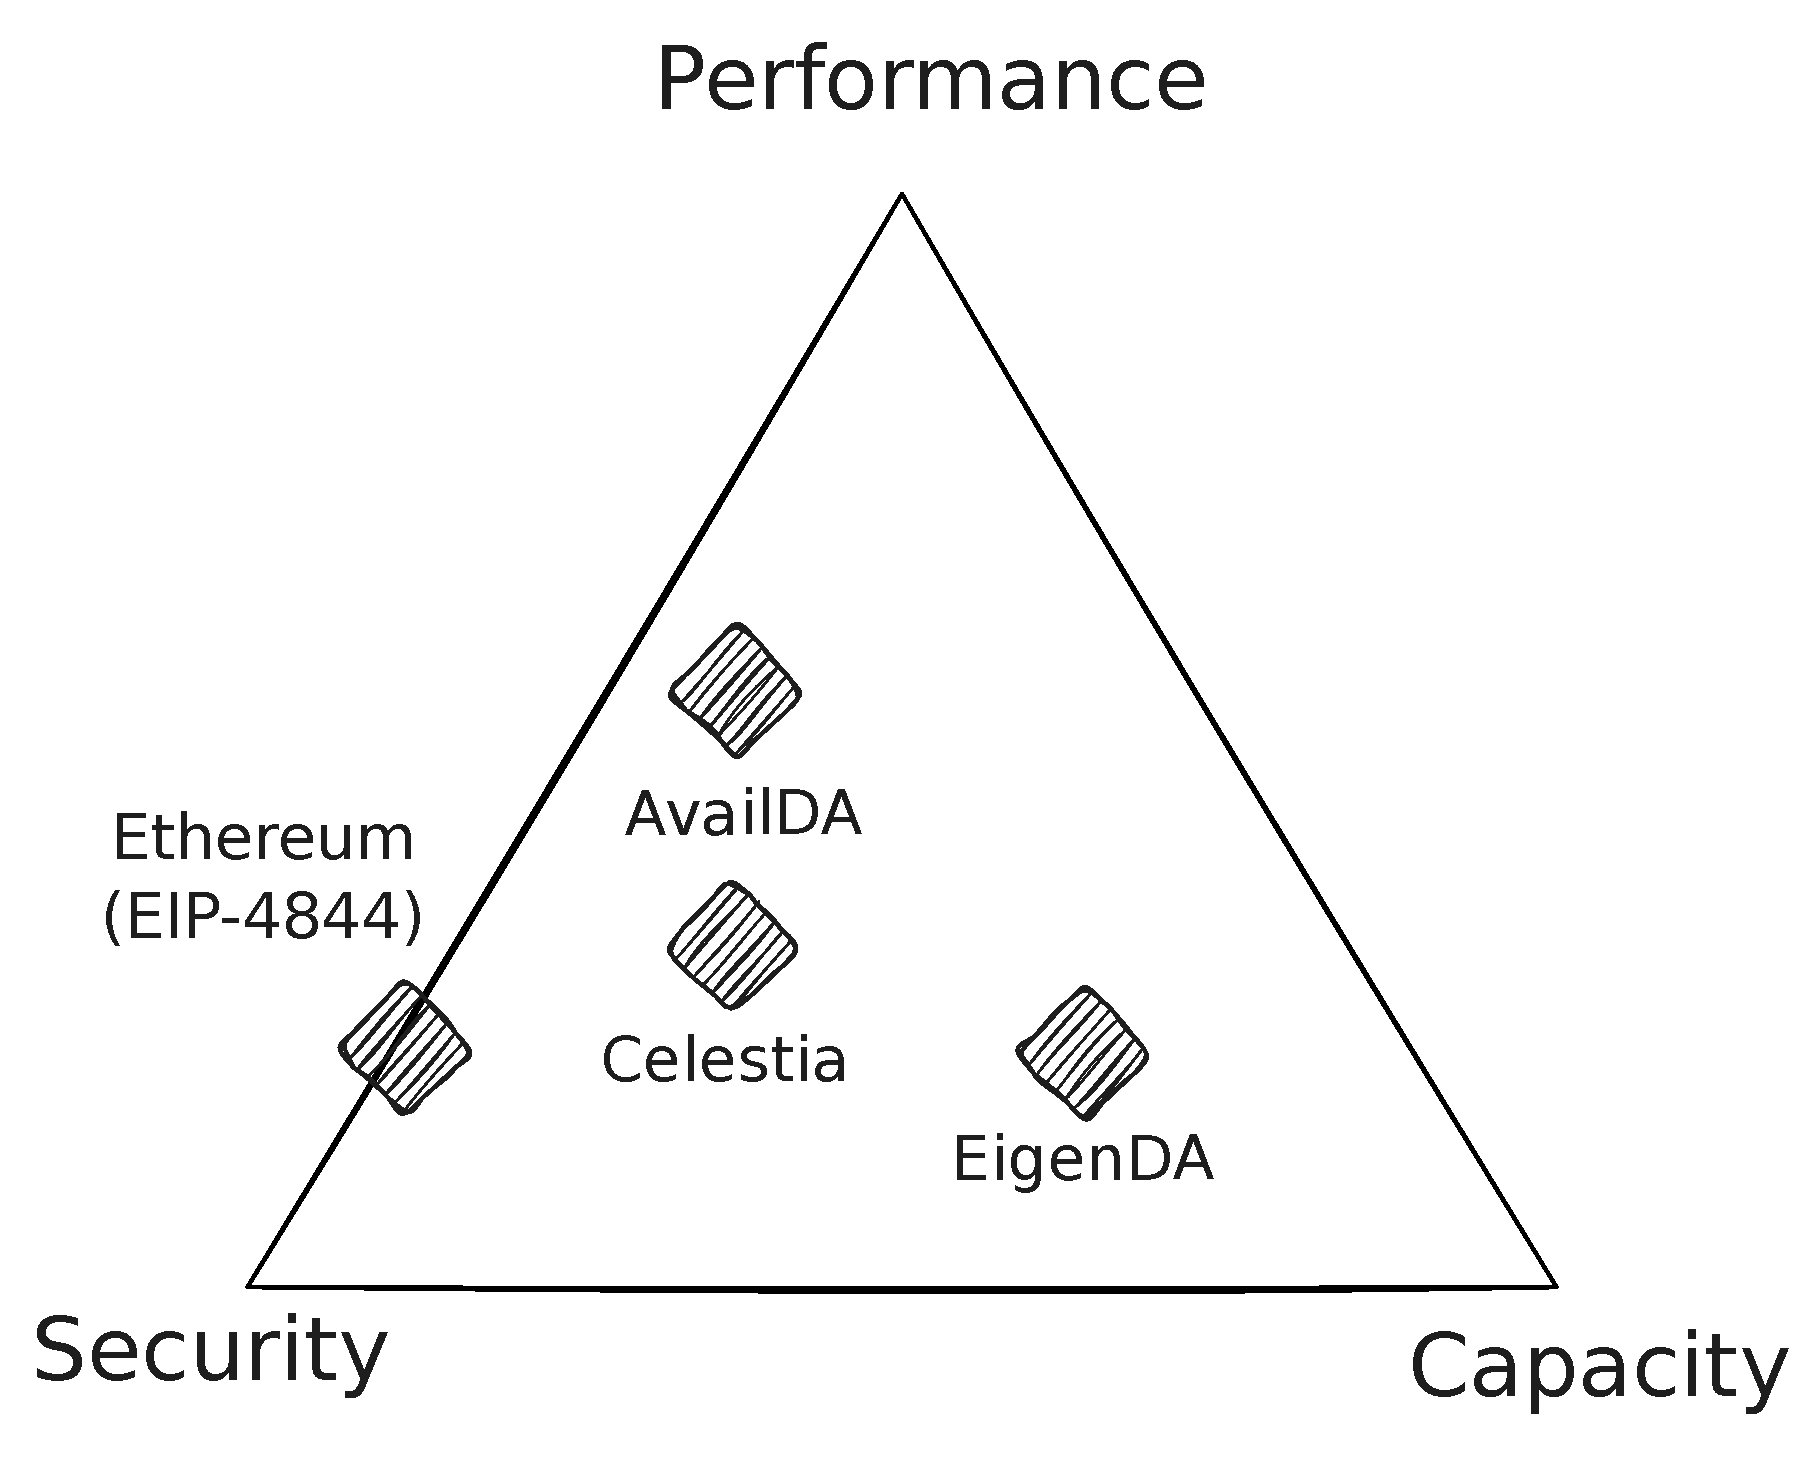
\includegraphics[scale=0.28]{da-trilemma.pdf}
    \caption{A representation of the Data Availability Trilemma considering Ethereum (EIP-4844), Celestia, AvailDA, and EigenDA.}
    \label{fig:da-trilemma}
\end{figure}

\paragraph{The problem of usability.} DA solutions that prioritize security need to give up in efficiency and scalability. Given that, current applications handling intensive data streams, such as AI protocols or on-chain games and DeFi are forced to adopt hybrid approaches, processing data offline and then using rollups to submit simple operations. Reducing the friction in the usability of Layer 2 and Layer 1 operations is a critical issue that needs addressing.
%
Fragmentation is also a primary issue. Currently, there are hundreds of L2s, each with its own tools, development stack, and interfaces. The rise of Rollups-as-a-Service (RaaS) and Appchains will jeopardize the entire ecosystem, leading to a disjointed user experience. Users must frequently switch networks to access different applications, resulting in a cumbersome and inefficient process that detracts from overall platform usability.
%
Lack of interoperability is another significant issue. In this fragmented ecosystem, ensuring seamless communication across different L2s is extremely challenging. The absence of a standardized, efficient cross-chain messaging and data transfer protocol forces users to navigate a complex landscape of bridging solutions that are often slow, costly, and sometimes vulnerable to security risks.

\subsection{Challenges}
Existing DA solutions face similar challenges, which we summarize as follows:

\begin{enumerate}
    \item Limited capacity: DA networks today have limited capacity for storing and verifying blobs. This limitation involves a security-performance-capacity tradeoff. To achieve adequate levels of security and performance, the number of blobs must remain constrained. Indeed, having excessively large blob spaces may lead to additional computation and communication overheads that undermine the correct execution of the protocol.
    \item Slow confirmation: Existing DA networks experience slow confirmation times, meaning the time required to finalize a data availability validation is prolonged. This issue arises from the communication complexity of DAS when executed on the consensus path. Specifically, when nodes need to check the data availability of certain blobs specified in a block, they either download the entire blob data or sample enough points to be convinced that the data is available (as proposed in Ethereum PeerDAS \cite{peerdas2024}). Both approaches result in extra communication complexity that requires additional back-and-forth messaging between involved parties. Consequently, the performance of the entire system is affected by higher latency.
    \item Fragmented ecosystem: To address the scalability problem at L1, numerous L2 rollup solutions have emerged \cite{crt:2024/889}. This has led to a fragmented ecosystem where applications are deployed on different L2s that cannot easily interact with each other, resulting in poor usability and a cumbersome user experience.
    \item Limited adoption: As a consequence of challenge 1, the DA adoption is nowadays limited to uses cases that do not have high-volume requirements in their applications. This limitation affects not only the throughput of DA layers but also compromises the broader vision of a massively adopted World Computer. Serving high-data demanding applications on the World Computer is today not possible. Use cases like AI protocols, on-chain games, and DeFi are forced to move parts of their processes off-chain and minimize blockchain components to smaller tasks.
\end{enumerate}

\subsection{The YoDA Approach}
YoDA aims to address these challenges by providing a DA solution that is faster, more secure, and significantly more developer-friendly. By introducing Instant Verifiable RAM (IVRAM), YoDA seeks to offer the fastest high-throughput memory component for the World Computer, accommodating a wide range of use cases and applications. It intends to leverage IVRAM to unify the fragmented L2 ecosystem, enhance interoperability, and deliver a seamless user experience comparable to more centralized platforms.

To achieve this goal, IVRAM combines a data sharding technique that distributes chunks of data blobs across different validators with a distributed blob building approach. The IVRAM draws from a decentralized network of nodes that run a BFT consensus protocol and FRI polynomial commitment techniques. In particular, users interact with the IVRAM by sending requests for storing their transaction data. Those pieces of data are then combined together into blobs and committed by the network in a resilient and decentralized manner. Blobs are encoded via erasure coding \cite{Geisel1990TutorialOR} to ensure high replication and fault tolerance, then a polynomial commitment scheme is used to ensure DAS and fast verifiability. The IVRAM nodes are responsible for accepting or rejecting blobs according to agreed consensus rules. We say that the data availability is finalized when the majority of IVRAM nodes reach consensus and approve the blobs. After that, users can query the network to counter verify the inclusion of certain transaction data or reconstruct the entire payload, without the need to trust any honest majority assumption in the IVRAM.

On top of the IVRAM, we develop additional services that enable high-capacity DA and unlocks new development paths by providing innovative data engineering interfaces and interoperability functionalities. In particular, YoDA promises to solve the challenges outlined above with the following objectives:

\noindent \textbf{Objective 1: IVRAM and Acceleration Layer for data-demanding applications.} This objective addresses challenges 1 and 2. To achieve this, we have two main contributions:
\begin{enumerate}
    \item Release of IVRAM as a Core Component of YoDA: The IVRAM is a fast and secure DA component capable of serving high-volume data streams with low latency without delaying confirmation of data availability finality.
    \item Pre-confirmations with Acceleration Layer: A pre-confirmation protocol built on top of the IVRAM allows optimistic confirmations of data availability to users before being published on the IVRAM.
\end{enumerate}

\noindent \textbf{Objective 2: Interoperability Layer for enhanced usability.} This objective introduces an interoperability service that leverages IVRAM to seamlessly move messages and data between rollups without introducing additional trust assumptions or middleware components.

\noindent \textbf{Objective 3: Interface Layer for DPS.} This objective aims to address challenge 4 by providing tools and services for DPS applications that deal with intense data workloads. The Interface Layer builds on top of the IVRAM and provides common interfaces similar to well-known streaming pipelining tools, caching, and storage platforms. By leveraging IVRAM, this layer promises to unlock DPS services that can be developed over familiar interfaces directly on the World Computer.
\smallskip

In the rest of this document, we will provide a high-level description of the YoDA protocol and how its core components meet the objectives. In the next section we provide an overview of the entire system, and present a simple data transaction flow.

\section{YoDA Architecture and Design}
YoDA is a decentralized data availability solution that offers high-throughput and low-latency storage for data blobs, along with unique services such as the Interface Layer, which implements DPS with standardized data engineering interfaces; the Interoperability Layer, which facilitates seamless L2 to L2 integration; and the Acceleration Layer, which enables near-instantaneous pre-confirmations.

\begin{figure}[htp]
    \centering
    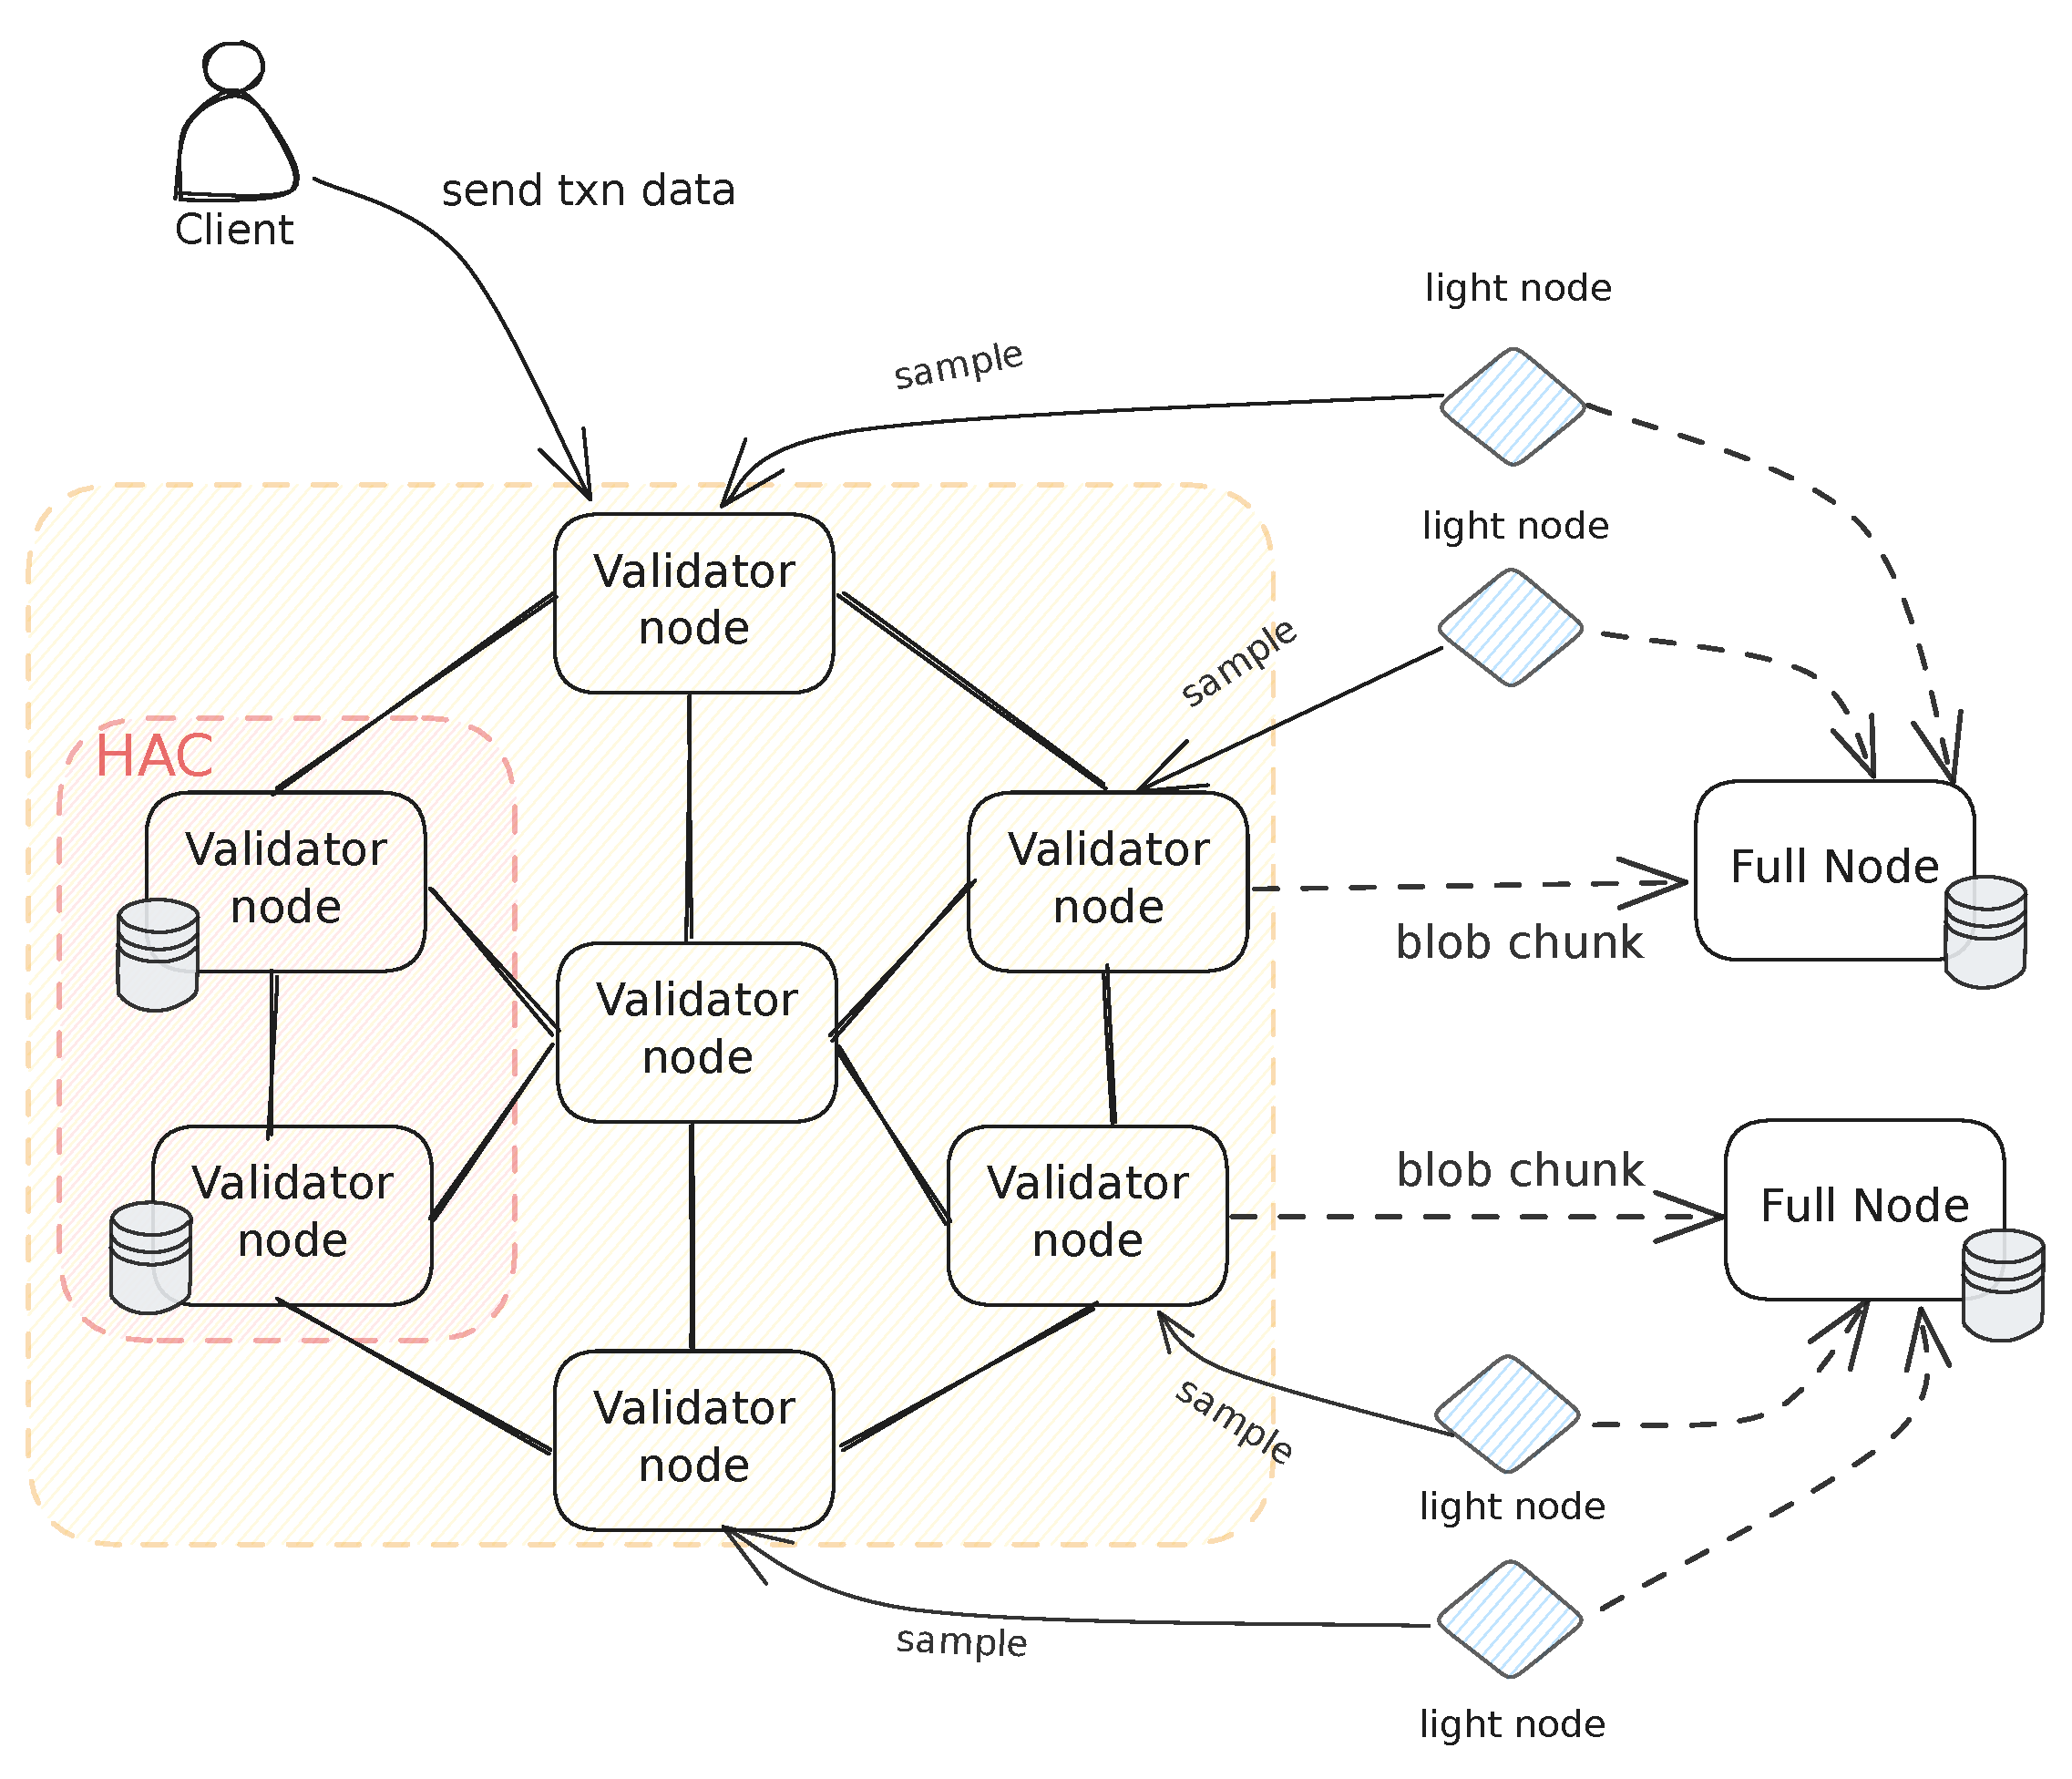
\includegraphics[scale=0.28]{yoda-net (1).pdf}
    \caption{The YoDA network.}
    \label{fig:yoda-net}
\end{figure}

Figure \ref{fig:yoda-net} illustrates the topology of the YoDA network and its principal actors:

\begin{itemize}
    \item \textbf{Validator Nodes}: Central to the IVRAM, these nodes receive transaction data from users and store them in blocks according to specific consensus rules. During consensus, a proposer is elected from among the validators to broadcast a new block containing a FRI commitment to the stored data. The remaining validators then verify this  commitment and either approve or reject the proposal accordingly. Validators participate in distributed blob building, ensuring both censorship resistance and expedited DAS confirmation. They are also eligible for selection into the High Availability Committee.
    \begin{itemize}
        \item \textbf{High Availability Committee (HAC)}: This is a fixed-size committee of validators (the size of which can be parametrized based on a performance-safety tradeoff) randomly selected for each slot. The committee downloads all blobs and verifies the correctness of the proposed block accordingly. It provides storage confirmation within consensus, delivering strong availability guarantees to the network.
    \end{itemize}
    \item \textbf{Full Nodes}: These high-performance nodes store full blocks with the entire data payload. Although they do not participate in the consensus protocol, they fetch data from validators and store full blobs data from the network. HAC members are also full nodes.
    \item \textbf{Light Nodes}: These resource-constrained nodes continuously query random samples of committed data to check their availability. They connect to at least one validator node and one full node. Upon verifying availability, they broadcast the received value to every connected full node, and store an ordered list of finalized block headers.
\end{itemize}

In a typical scenario, each client application represents an L2 rollup aiming to make its transaction data available for L1 verification. Clients submit their transaction data to validators, which organize it into chunks. A distributed blob building process (described in the next section) is then initiated. During this process, an elected proposer assembles the final blob from the chunks provided by other validators and proposes it for final approval. Once consensus is achieved, validators confirm data availability and distribute their chunks to connected full nodes. Light nodes assist in the reconstruction process by querying random samples from validators and broadcasting them to full nodes. After collecting a sufficient number of queries, any full node can reconstruct the complete data from the network.

\paragraph{Blobs Transaction and Block Lifecycle.} A data transaction is the unit of data for which client applications seek to make available. It represents the data of a transaction executed on the L2. These transactions are organized into blobs and periodically stored on the IVRAM with a new block. The lifecycle of a blob transaction along with the block proposal is as follows:

\begin{enumerate}
    \item Data submission: clients submit transactions data to at least one validator node and wait for DA confirmation.
    \item Distributed blob building: a proposer, elected from the IVRAM validators, receives transaction data from other validators and encodes them together into blobs. Afterwards, the proposer computes a Merkle commitment to that blobs by running FRI, and with that commitment assembles a new block for the IVRAM. The block includes the commitment along with additional metadata. The full transaction data is not included, and remains sharded across multiple validators.
    \item Validators receiving a DA block check if their data has been included in the commitment. If a majority agree, the block is verified. Validators participating in the consensus protocol are also responsible for storing transaction data that the block commits to.
    \item Optionally, some validators can elect themselves as HAC members by running a random beacon. When approving a block proposal, they provide proof of membership to the current HAC to the proposer. Thus, members receive all block data; however, given that HAC is of constant size, communication overhead remains negligible.
\end{enumerate}

\section{Technology Components}
YoDA is a comprehensive, multi-layer technology stack comprising four core components: the IVRAM Layer, Acceleration Layer, Interface Layer, and Interoperability Layer. The IVRAM integrates validator nodes, full nodes, and light nodes, all operating under a novel consensus mechanism. This robust foundation enables YoDA to deliver advanced functionalities across its Acceleration, Interface, and Interoperability Layers, ensuring seamless performance and integration.

\begin{figure}[htp]
    \centering
    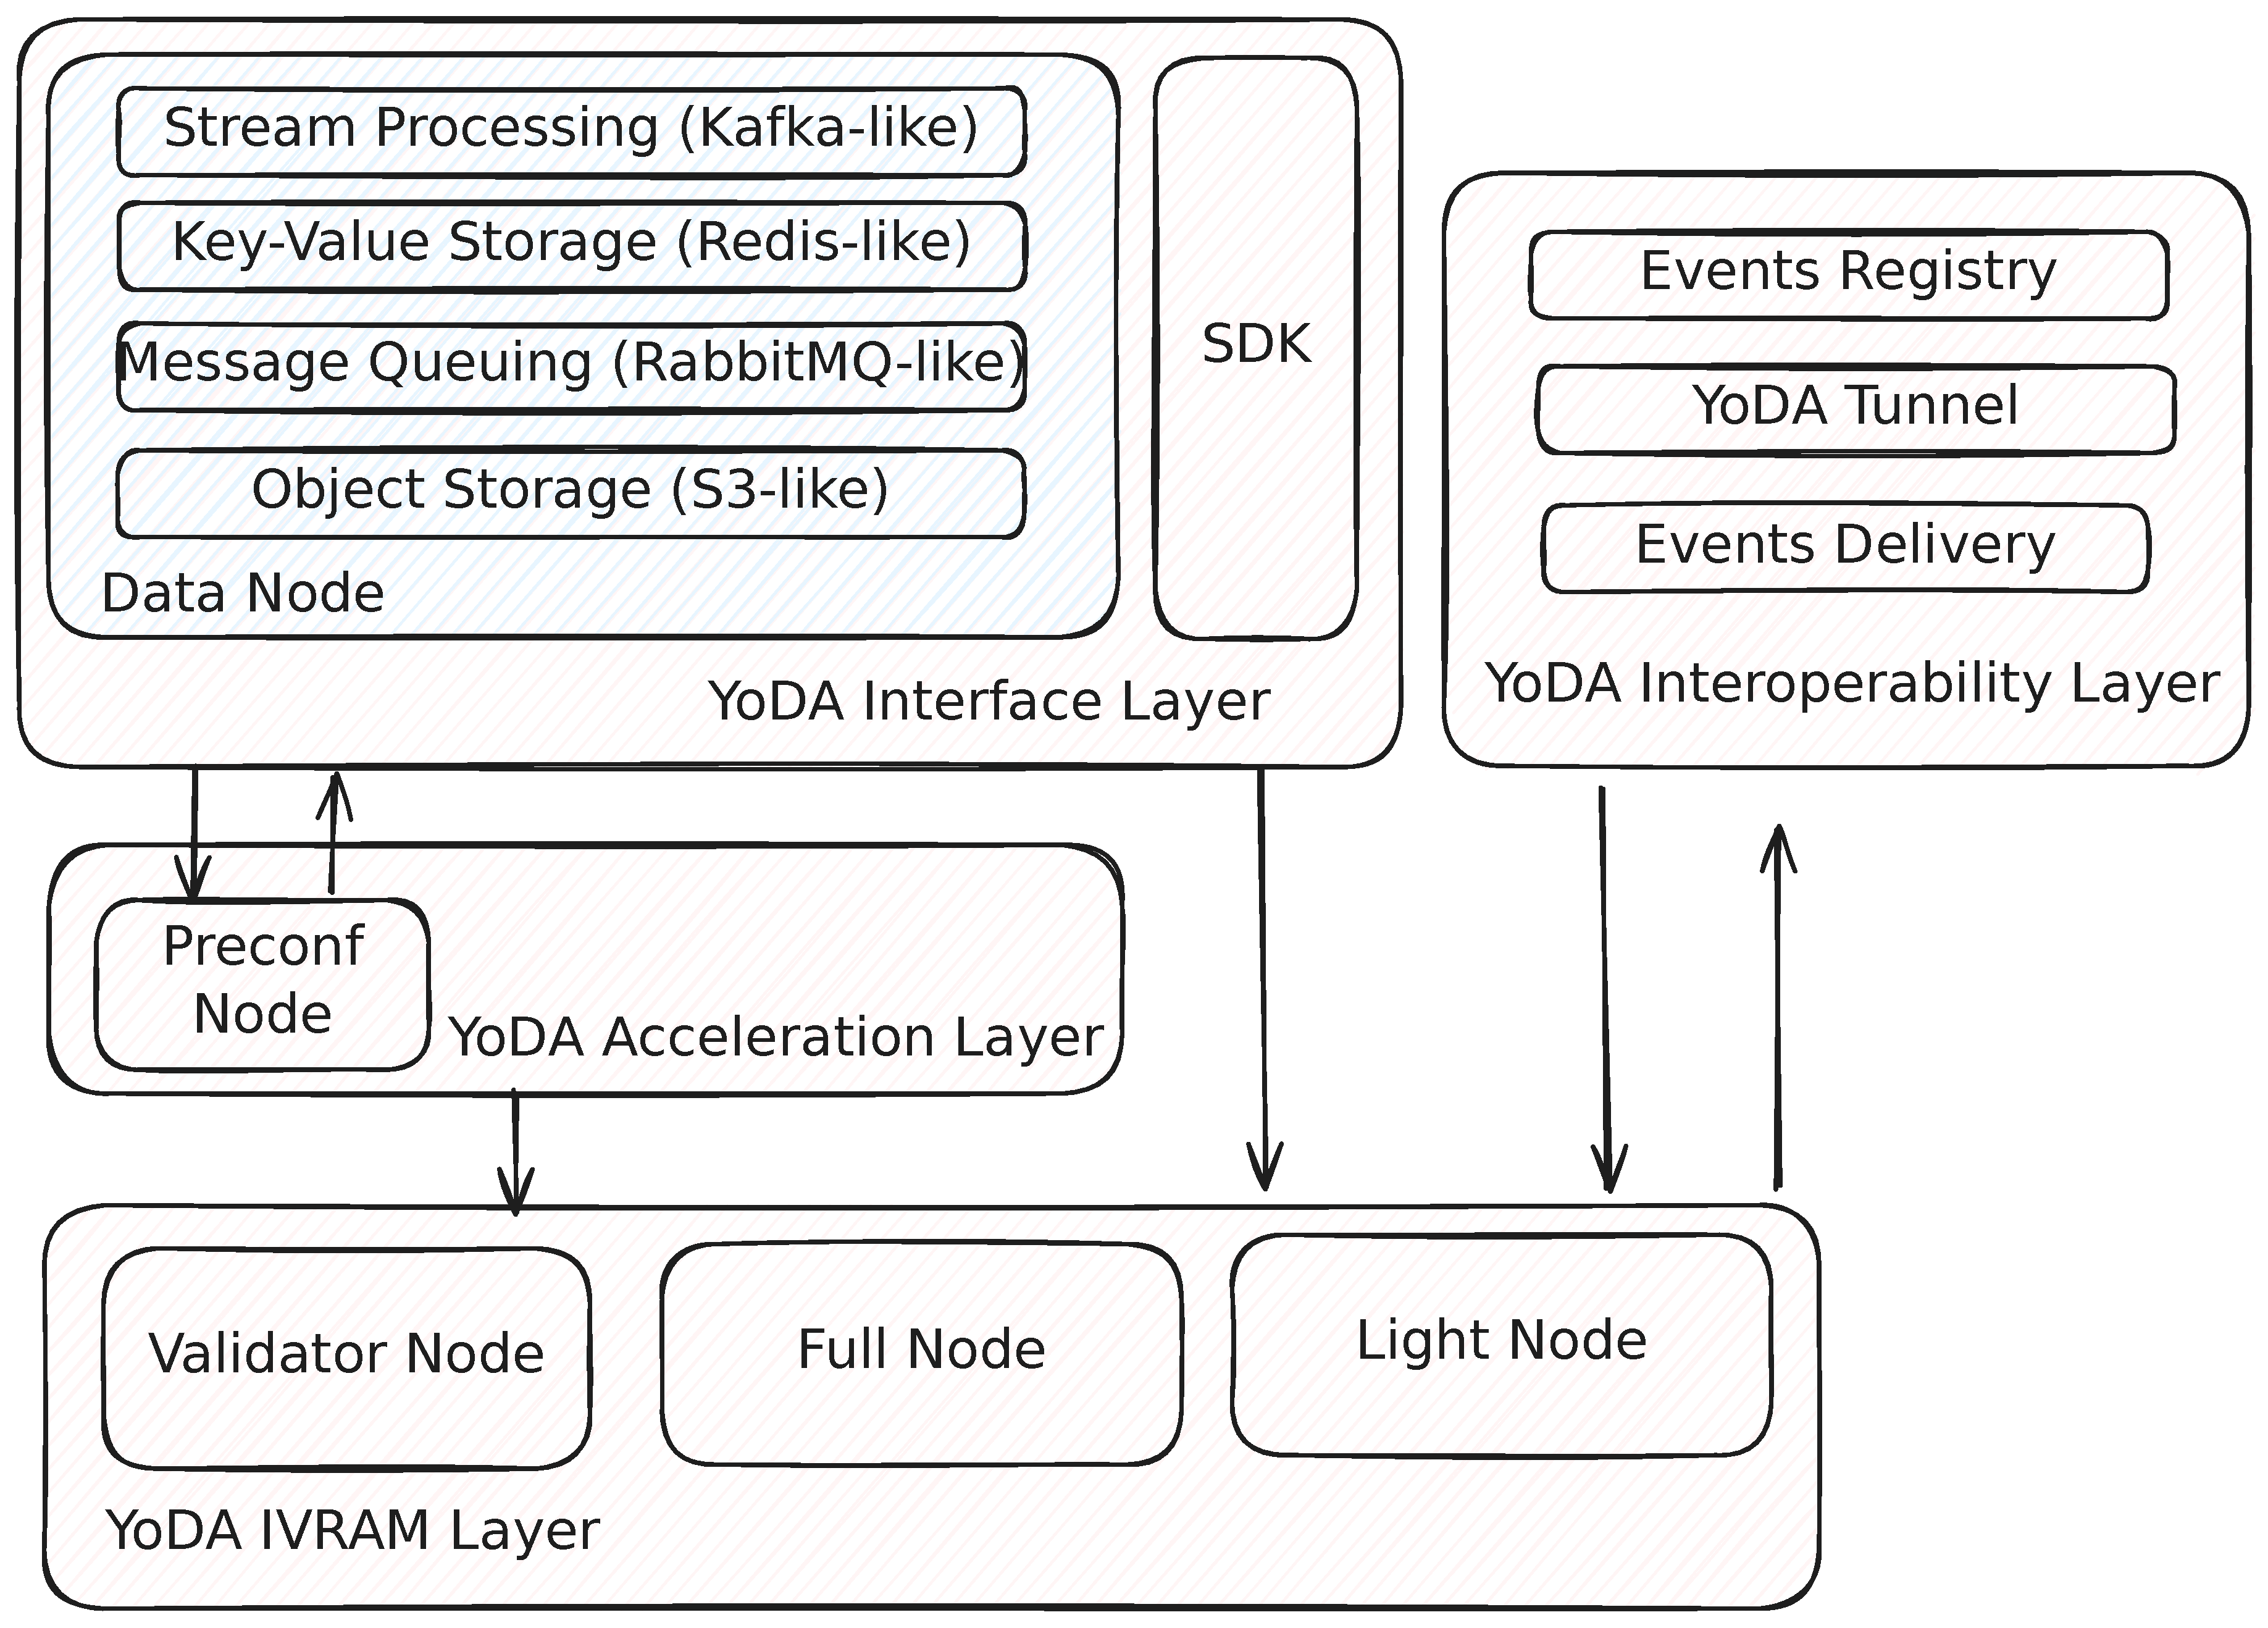
\includegraphics[scale=0.2]{yoda-arch.pdf}
    \caption{The YoDA multi-layer technology stack}
    \label{fig:yoda-arch}
\end{figure}

Figure \ref{fig:yoda-arch} illustrates the multi-layer stack of the YoDA system and demonstrates how its various layers interact. When a data block enters the IVRAM Layer, validator nodes verify the correctness of its associated FRI commitment. However, due to the finality latency inherent in the consensus protocol—particularly when large data blobs are involved—reaching consensus on erasure coding commitments can be time-consuming. The Acceleration Layer addresses this by introducing pre-confirmation nodes that expedite verification. By assuming an optimistic finality for submitted data, this setup allows for real-time confirmation. Once verified within the IVRAM Layer, the Interoperability Layer facilitates seamless communication between rollups via light nodes using the YoDA tunnel.

To enhance developer accessibility, the Interface Layer offers seamless integration by featuring data nodes that emulate popular Web2 data engineering tools and SDK components supporting multiple programming languages.

\subsection{Instant Verifiable RAM}
The Instant Verifiable RAM (IVRAM) is the core innovation of YoDA, serving as a low-latency, instant-finality DA layer that provides validity proofs. IVRAM functions as a form of temporary, verifiable storage that is both fast and secure. It ensures instant data availability confirmations, providing assurance that once data is stored, it cannot be altered or reversed. This feature is critical for applications where timely and reliable data availability is essential. By utilizing FRI commitments, IVRAM ensures that all stored data is verifiable, meaning any party can check the integrity and availability of the data without needing to trust the data provider, nor downloading the full blobs.

\subsubsection{Distributed block building}
The IVRAM interprets transaction data as blobs. These blobs are encoded into an extended payload using erasure coding, a technique that divides data into fragments and encodes these fragments with redundant data, known as parity data. The fragments are distributed across multiple storage nodes, allowing for the reconstruction of the original data even if some fragments are lost or corrupted.
%
Within the IVRAM, the extended blob is divided into pairs of chunks and parity chunks. Each pair is then allocated to a specific validator. In the distributed blob building model, for each proposal, validators provide parts of the blobs to an elected proposer who then computes the erasure coding and commitments, i.e. FRI polynomial commitments. Consequently, when a new consensus proposal is made, there is no need to send data back and forth between validators and proposers. Instead, each validator samples portions of their commitment via DAS and verifies that their data has been correctly included. This optimization allows IVRAM to achieve high speed and large data throughput without introducing communication overheads during consensus agreement.

\subsubsection{Consensus rules}
At the core of YoDA’s IVRAM is a BFT consensus protocol executed by validators. To store blobs in the IVRAM, validators must agree on a blockchain data structure where each block contains a FRI commitment to some erasure-coded data. If the consensus correctly terminates, the block is deemed valid and DA is confirmed. The adopted consensus protocol ensures:
\begin{enumerate}
    \item Safety and liveness under adversarial conditions: The committed data must remain secure even in the presence of an honest minority or network issues.
    \item Instant finality: Once validators approve a proposal, they also verify the block’s availability, which is then considered finalized and irreversible (except in cases of hard forks).
\end{enumerate}

To meet these requirements, we have chosen a partially-synchronous BFT protocol that operates under the assumption of $n=3f+1$ online validators, where $f$ can be malicious and $2f+1$ are honest. A majority of validators are required to check the block’s correctness to ensure strong integrity of committed data and high availability guarantees, even if some nodes are offline.

\subsubsection{DAS and retrievability}
In the IVRAM, there are two phases during which a node is particularly interested in sampling: (i) during consensus validation and (ii) during light nodes DA verification.

\paragraph{DAS during consensus.} Figure \ref{fig:yoda-das} provides a graphical representation of the DAS executed along the consensus path. When a new extended blob is proposed, validators sample random points within their allocated chunk and verify the correctness of the provided FRI commitment concerning those points.

\begin{figure}[htp]
    \centering
    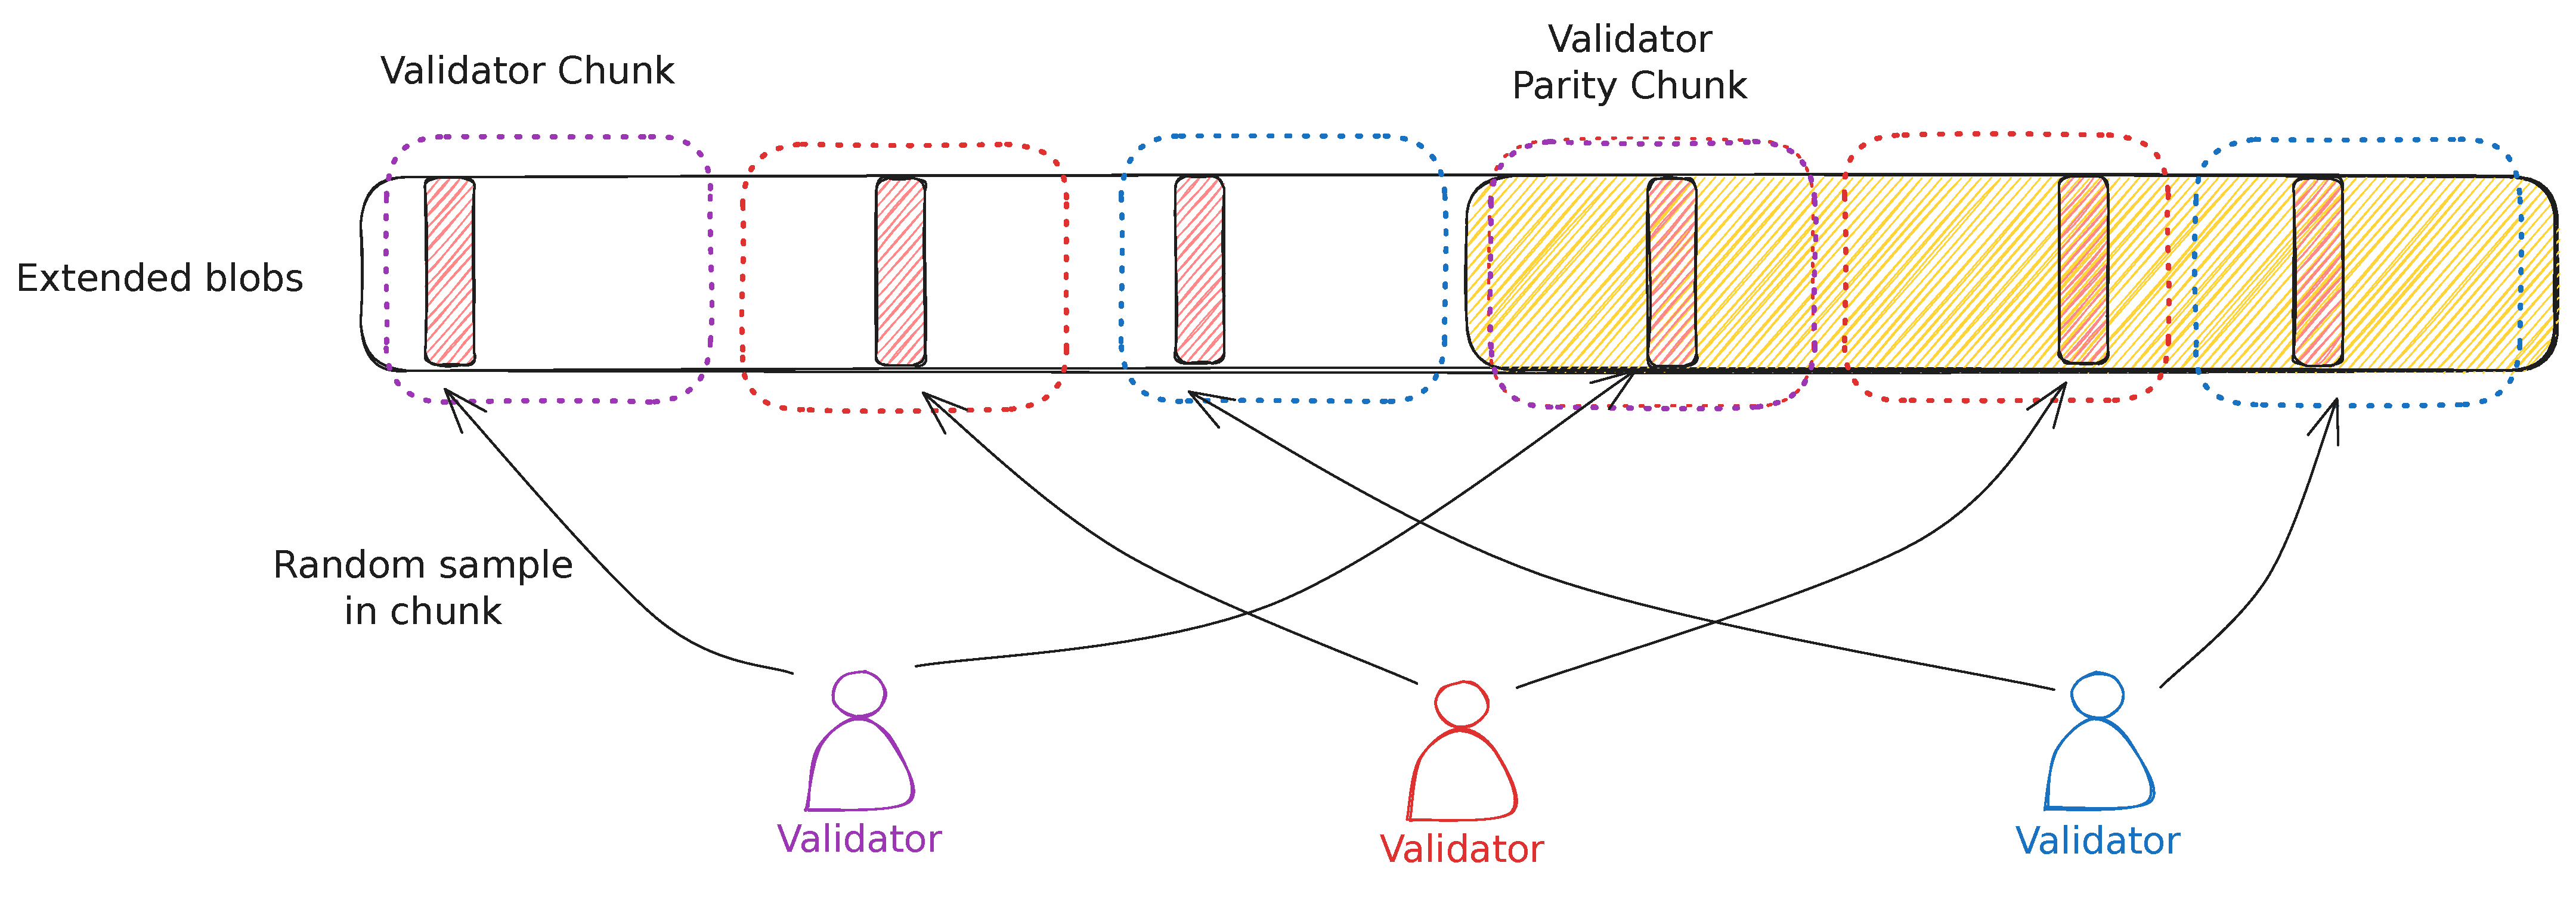
\includegraphics[scale=0.2]{das-ivram.pdf}
    \caption{An example of DAS on the IVRAM with three validators.}
    \label{fig:yoda-das}
\end{figure}

\paragraph{DAS for light nodes verification.} Light nodes sample random points from the extended blob by querying one or more validators. After a sufficient number of samples, light clients can consider the data available and pass the verification test. Otherwise, they will query a HAC member for the missing parts of the data. If those nodes fail to respond, a recovery mechanism is activated, which must be defined via governance rules and social consensus. This approach allows light nodes to check availability without relying on an honest majority.

\paragraph{Retrievability.} Light clients begin sampling DA blobs to ensure sufficient confidence that the data is available. To retrieve a sample, the light client maintains a connection to validators, from whom it can request samples footnote. A DHT-based peer discovery mechanism will allow nodes to connect with a sufficient number of validators that store the chunks of blobs they want to sample. When sampling, the light node receives the sample data plus a proof that verifies its inclusion in the claimed commitment.
%
To fully verify data availability, the light node may query validators until it has collected enough samples to reconstruct the original data from a DA block. This strictly depends on the encoding configuration used, but generally speaking, at least half of the extended payload is required for reconstruction.
%
Reconstruction is typically expected to occur on full nodes, which have greater computational resources. To this end, light nodes that retrieve samples broadcast their results to connected full nodes (at least one) for reconstruction. In addition, full nodes receive chunks of data blobs from validators. When a sufficient number of data points is retrieved, then the full node can reconstruct the data.

\subsection{Interface Layer}
The YoDA system offers developer-friendly interfaces that integrate popular tools like Kafka, Redis, and RabbitMQ into a decentralized framework. This enables developers to use familiar APIs. The Interface Layer consists of two main components: the Data Node Component, which collaborates with full and light nodes to emulate these widely used tools, and the SDK Component, providing development kits in languages such as Python, Go, Rust, C++, Java, JavaScript, Scala, and Unity/C\# for seamless integration across various programming environments.

The Data Node provides interfaces that decentralized applications can use to interact with data engineering tools familiar to Web2 developers. For example, with capabilities similar to Kafka and RabbitMQ, applications can leverage publish-subscribe mechanisms for various decentralized use cases. These include accessing L2 data via app-specific IDs within the IVRAM and enabling messaging across different L2 networks to ensure seamless data flow. This facilitates smooth interaction across on-chain applications and bridges the gap between Web2 and Web3 applications. By accessing the node APIs, a Web2 system can easily subscribe to on-chain app-specific data streamed from the IVRAM.
%
An illustrative example is shown in Figure \ref{fig:yoda-interface}, where Web2 centralized servers efficiently pull data from different rollups (and vice versa).\footnote{This example assumes that the L2 rollups trust the Web2 data providers, for instance, by authenticating messages using a pre-registered public key.} In this example, rollups publish data to the IVRAM using the PubSub endpoint of a DA Node. Each publish event is identified by the tuple $(rollup_{id}, app_{id})$ where the first element specifies the rollup's ID and the second represents the PubSub topic. To subscribe, servers need to specify the list of topics they wish to register for.

\begin{figure}[htp]
    \centering
    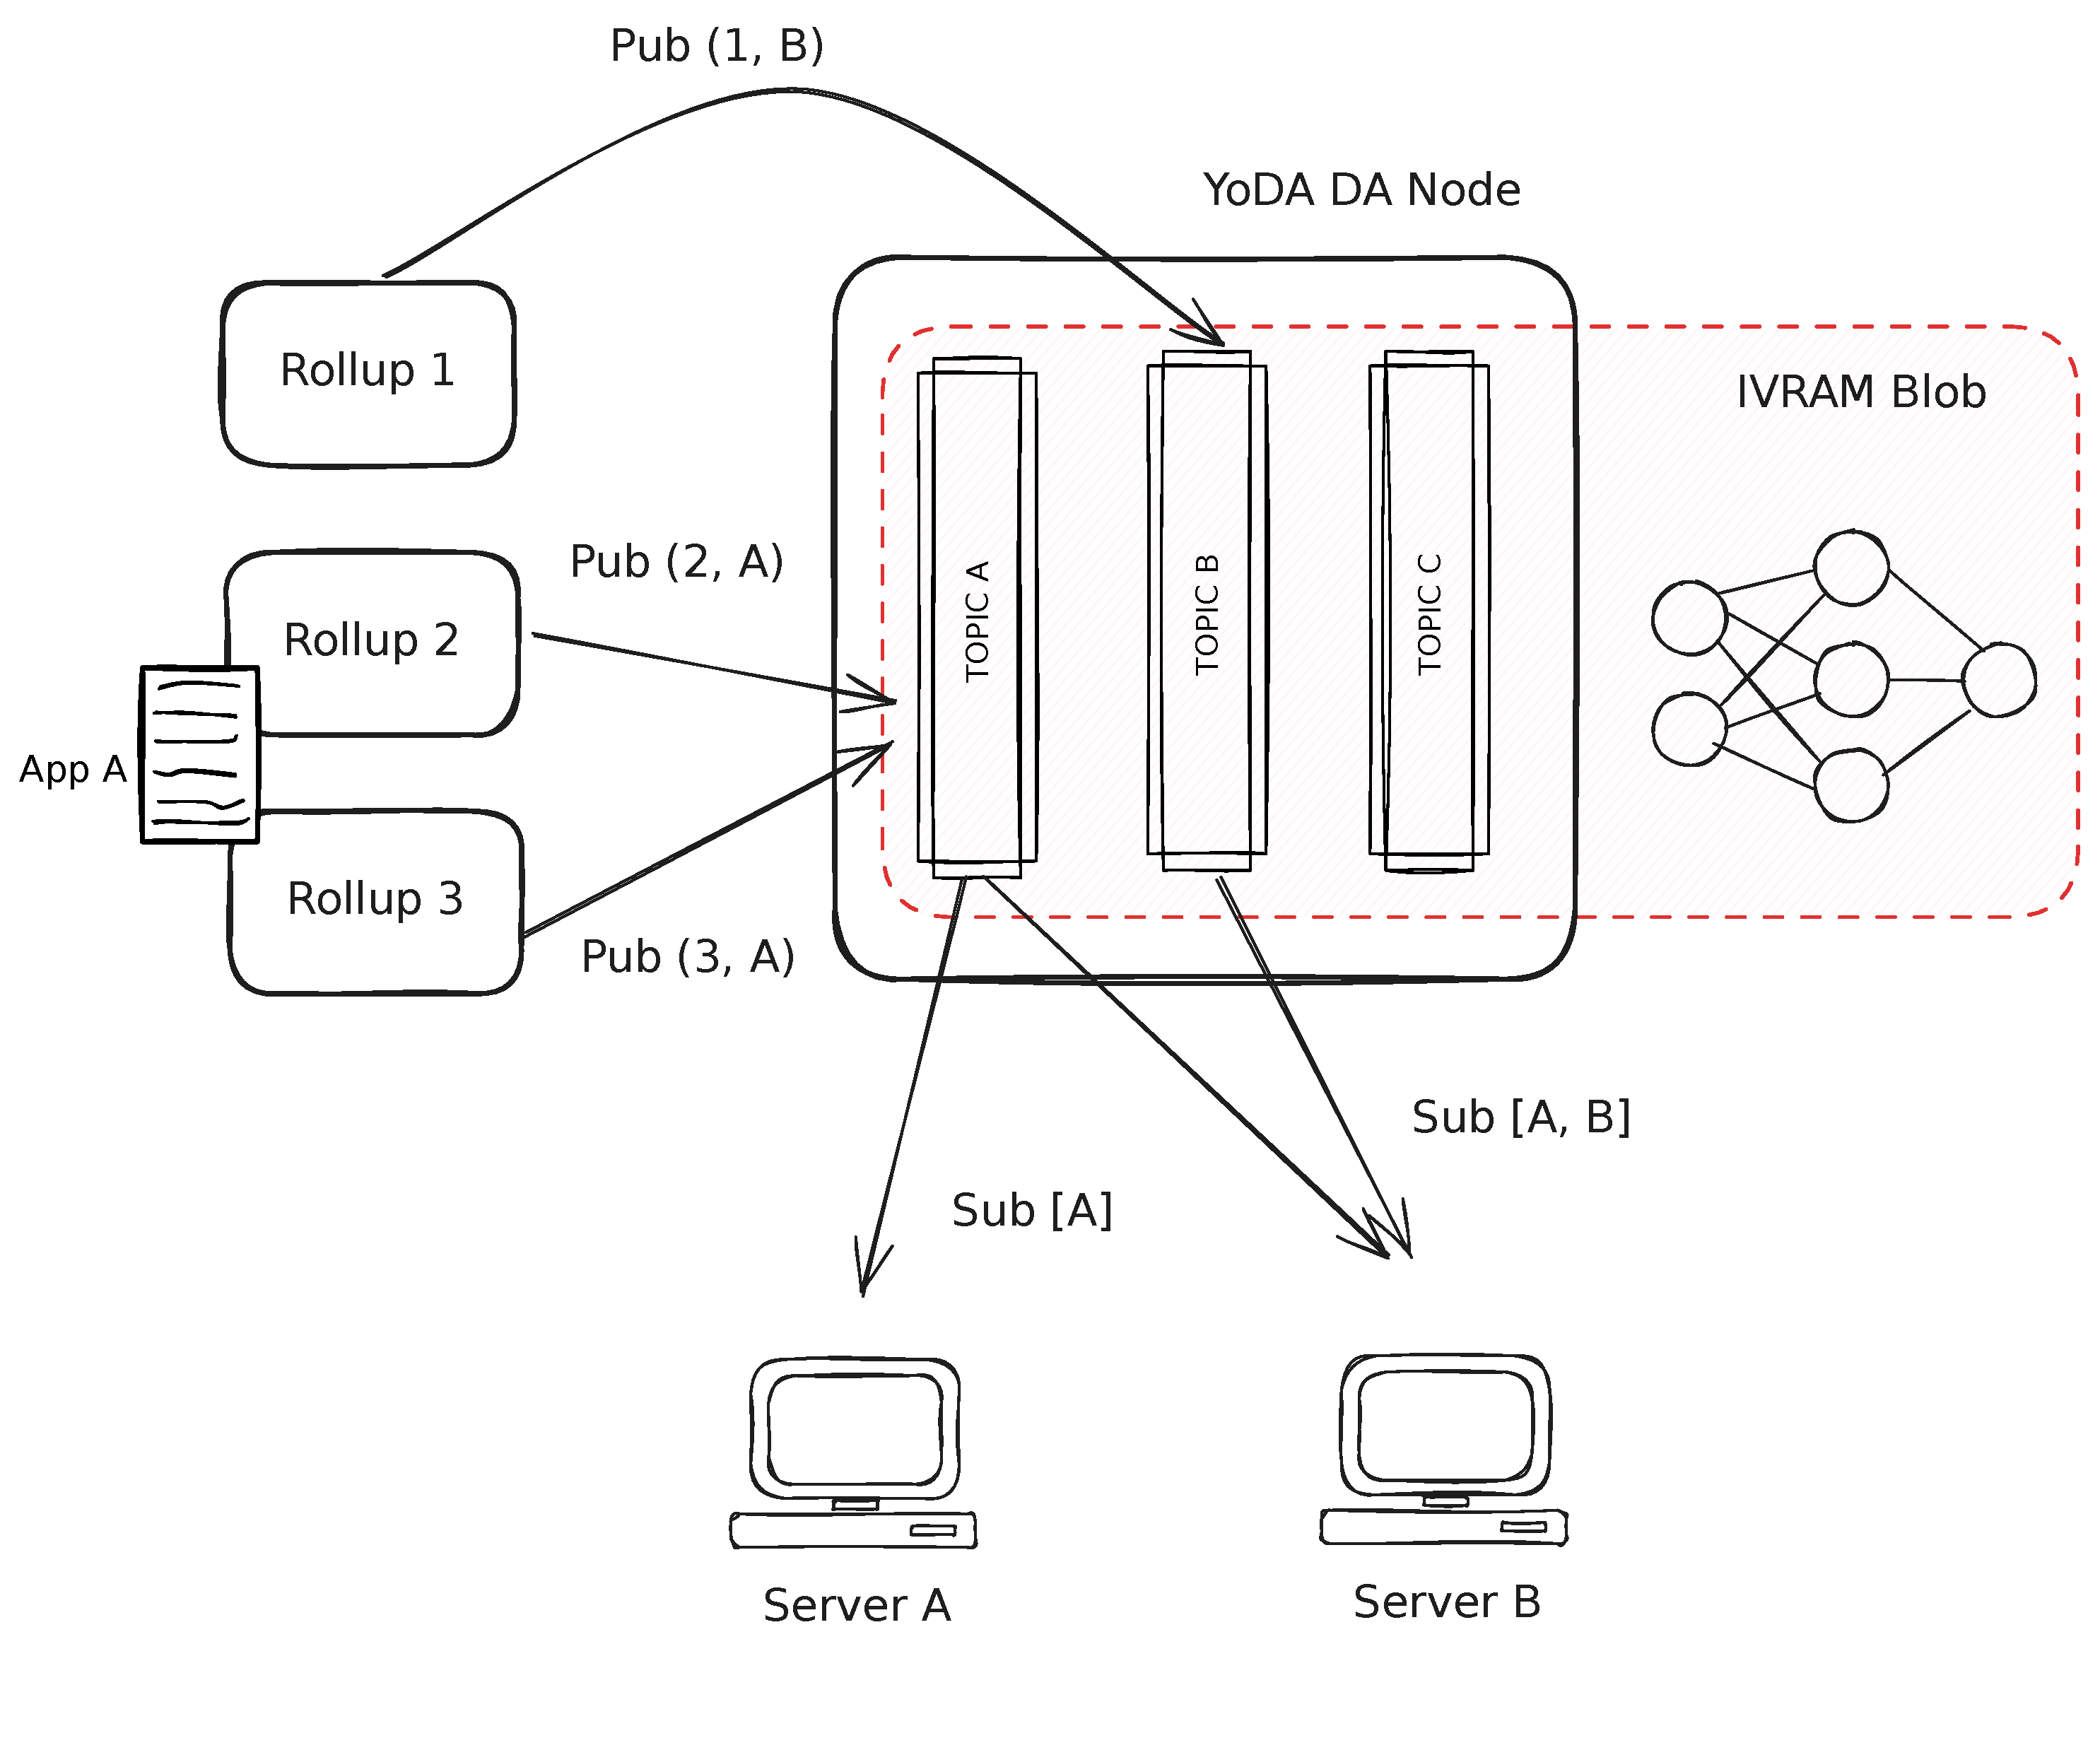
\includegraphics[scale=0.2]{we2-web3 (1).pdf}
    \caption{An example of YoDA PubSub workflow from three rollups and two web2 servers.}
    \label{fig:yoda-interface}
\end{figure}

For Redis-like key-value storage, the node acts as a global cache, providing rapid data access and retrieval for decentralized applications. Additionally, for applications requiring Oracle Request for Access (ORA)-like reliability, the Redis-like component offers configurable data retention policies tailored to specific needs, like Amazon S3 expiration policies.
%
Complementing the Data Node Component, the SDK Component provides software development kits that simplify integration into decentralized applications. Available in multiple programming languages—including Python, Go, Rust, C++, Java, JavaScript, Scala, and Unity/C\#—these SDKs enable developers to seamlessly connect with both the IVRAM and full node components. This multilingual support allows developers to build on YoDA’s platform using familiar tools and codebases and easing the transition from traditional to decentralized systems. The SDK Component thus enhances YoDA's accessibility and adaptability across a wide range of technical environments.

\subsection{Interoperability Layer}
The Interoperability Layer is a cross-rollup communication protocol that leverages YoDA IVRAM to securely validate and store messages between rollups and appchains. It allows direct and efficient interactions across chains without relying on additional trust components like bridges or multi-signature setups.
%
At the core of the interoperability layer there is the Message Registry, a special portion of the IVRAM that stores L2-to-L2 interoperability messages. The registry on the IVRAM makes interoperability efficient on both the dispatching side of the message, and the retrieval.
%
To dispatch an interoperability message, users use a special transaction type that stores app-specific interoperability events. It requires users to specify two parties, the Source and the Destination of an interoperability message. In addition, the transaction must specify the content of the message, e.g. move data element from Source to Destination, interacting with a smart contract on the Destination, etc.  
%
To retrieve an interoperability message, the Destination L2 can monitor the IVARM Message Registry and retrieve interoperability messages on their path. When a new message appears, it can be verified by and executed accordingly.

The YoDA Interoperability Layer supports two use cases: (i) native L2s interoperability and (ii) non-native L2s interoperability. The former case allows rollups or appchains to directly interact with the Message Registry and access cross-chain data seamlessly. In the latter, a relay node will be required to submit and retrieve events from non-native L2s to the IVRAM.

Another crucial component of the Interoperability Layer is the YoDA Tunnel, i.e. an L1 component that brings the IVRAM state on the L1 for fast DA verification. The Tunnel gathers finalized DA commitments from the IVRAM using a trust-minimized, proof-based light client deployed as an L1 smart contract.

\subsection{Acceleration Layer}
The Acceleration Layer serves as an optional yet critical component for applications demanding real-time data access and swift processing. Applications can achieve enhanced performance through the provision of pre-confirmation for data payloads, effectively reducing latency and improving user experience. This layer operates by aggregating application transaction data into manageable batches, which are optimistically assumed to be available and then systematically submitted to the underlying YoDA IVRAM. The entire process is managed by specialized entities known as the Preconf Nodes (also known as Delegated Preconfer in literature \cite{drake23}).
%
One of the key advantages of the Acceleration Layer is its ability to minimize DA verification waiting times. This strategy allows users to interact with the application seamlessly, without the inevitable delays typically associated with consensus mechanisms.

The Preconf Node serves as a pivotal component designed to ensure rapid pre-confirmation of submitted application data. The Preconf Node functions by temporarily storing incoming data for brief periods, during which it organizes and batches the data to optimize submission efficiency. Once data is batched to a standard size, the Preconf Node forwards the data to the next proposer of the IVRAM, ensuring that the transition from pre-confirmation to finalization is both swift and reliable.
%
In traditional L1 designs, pre-confirmation is provided by the block proposer, who guarantees the inclusion of transactions in the next block. However, in our case, we propose to introduce a mempool populated by the Preconf Nodes. Validators among preconf Nodes in this mempool will include these pre-confirmed data batches in the chunk they build. This design ensures that pre-confirmed data is selected for inclusion in the following block, effectively combining the pre-confirmation efficiency with the security of the IVRAM layer.

\section{Market Potential}

\subsection{Interoperability Market}
The interoperability market is experiencing rapid growth due to the proliferation of blockchain networks and the need for cross-chain communication. LayerZero reports revenue of \$16 million per year, with 140\% growth in 2023 \cite{layerzero_labs_2024}, and Chainlink CCIP achieved \$484,000 in revenue shortly after launch, with 180\% growth over two months \cite{chainlink_ccip_2024, newsbtc_chainlink_2024}. There is a strong demand for reliable, secure, and efficient cross-chain messaging solutions. YoDA's advanced features and faster, more secure messaging capabilities make it well-suited to capitalize on this market opportunity.

\subsection{Web3 Infrastructure Market}
Web3 infrastructure providers generate significant revenue and are essential to the growth of the decentralized ecosystem, with combined revenues exceeding \$100 million per year \cite{wifi_talents_web3_statistics}. By integrating with RaaS and RPC providers like Conduit, Caldera, Alchemy, and QuickNode, YoDA can tap into existing customer bases and distribution channels. As more developers build decentralized applications, the demand for robust infrastructure will continue to rise. By positioning itself within this market, YoDA can leverage its competitive advantages to gain market share and drive adoption.

\subsection{DA Layer Market}
The Data Availability layer market is poised for significant growth as modular blockchains and rollup architectures become more prevalent. Current market indicators include Celestia's estimated revenue of \$7.2 million per year, with a fully diluted valuation of \$6.8 billion \cite{growjo_celestia_labs}. Growth drivers include increasing adoption of Layer 2 solutions, demand for scalable blockchain infrastructure, and the need for efficient data availability mechanisms. YoDA's superior performance and security position it to capture a substantial share of this expanding market, offering an attractive alternative to existing solutions.

\section{Related Works}
\textbf{Data Availability Layers.} Decentralized Availability (DA) layers such as Celestia, Avail, and EigenDA offer different approaches to securing data availability in blockchain ecosystems. Celestia uses an optimistic DA model that allows fraud proofs. It achieves a block time of 12 seconds, but finality depends on fraud proof resolution, which adds a delay. Avail relies on KZG validity proofs, providing a more structured verification. It has a 20-second block time and approximately one-minute finality, balancing verification correctness with moderate finality speed. EigenDA, with its permissioned data dispersal model and integration of Ethereum’s slower finality, prioritizes security over speed. This approach leads to around 15 minutes for data finality, due to additional trust assumptions on top of Ethereum \cite{avail_dal_guide}. YoDA adopts FRI validity proofs, achieving confirmation within 2-3 seconds and potentially as fast as 200 milliseconds with pre-confirmations. Unlike Celestia, Avail, and EigenDA, YoDA’s design emphasizes both fast finality and accessible data availability. This approach makes it suitable for applications requiring immediate data confirmation alongside reliable verification mechanisms.

\textbf{Data Engineering Tools.} Centralized cloud services offer essential tools for Web2 data engineering, including Kafka, Redis, and RabbitMQ. These services provide managed infrastructure with built-in scalability and security. Kafka enables real-time data streaming, allowing applications to process data as it arrives. Redis provides in-memory caching for fast data access, improving performance in high-traffic applications. RabbitMQ handles message queuing, ensuring reliable communication between services. While these tools offer scalability and reliability, they rely on centralized control, which can limit transparency and decentralization. YoDA offers a decentralized alternative that is developer-friendly and integrates with these popular tools, making it an attractive option for developers focused on building decentralized applications requiring robust data engineering capabilities.

\section{Conclusion}
YoDA represents a significant advancement in the field of data availability solutions for decentralized applications. By integrating Instant Verifiable RAM (IVRAM) with quantum-safe FRI commitments, YoDA addresses the critical challenges of speed, security, and developer accessibility that have limited the scalability and user experience of blockchain networks. By offering familiar data engineering interfaces, YoDA lowers the barrier to entry for developers, fostering innovation and seamless integration into existing workflows. Its focus on temporary, verifiable storage optimizes performance and cost-efficiency for applications that require fast and secure data handling, such as gaming, AI, and cross-chain DeFi.
%
With a robust architecture that ensures instant finality and low latency, YoDA is well-positioned to become the preferred DA solution for Web3 builders. Its competitive advantages in speed, security, and developer experience make it a compelling choice for those seeking to harness the full potential of decentralized technologies. By addressing the fragmentation and inefficiencies of the current Ethereum ecosystem, YoDA paves the way for a more unified, scalable, and user-friendly decentralized landscape, driving the next wave of decentralized application development.

% Bibliography section 
\clearpage 
\printbibliography

\appendix
\section{FRI Commitments}
FRI (Fast Reed-Solomon Interactive Oracle Proof of Proximity) \cite{bensasson18} is a protocol used to verify that a polynomial has a low degree without revealing the polynomial itself. It is commonly employed in zero-knowledge proof systems, such as STARKs, to ensure that a prover’s commitment corresponds to a polynomial of bounded degree. FRI works by encoding the polynomial as a Reed-Solomon codeword \cite{Geisel1990TutorialOR} and committing to it using Merkle trees. The verifier can then query specific parts of this commitment to check proximity to a low-degree polynomial, making the process efficient and scalable.

A cornerstone of YoDA's architecture is its use of FRI to verify that data is correctly encoded and available without requiring the verifier(s) to download the entire payload. Unlike the KZG polynomial commitment scheme, FRI is bases on hash functions and thus considered quantum-safe \cite{zych2018quantum}, which is crucial as quantum computing advances and poses potential threats to cryptographic systems based on traditional algorithms. Additionally, FRI commitments eliminate the need for a trusted setup phase, reducing potential vulnerabilities associated with initial parameter generation. Finally, computing FRI proofs is significantly faster than those based on KZG schemes, contributing to the low-latency characteristics of YoDA.

\section{Byzantine Fault Tolerant Consensus}
Byzantine fault-tolerant (BFT) consensus is a method used in distributed networks to achieve consensus even when some nodes may act maliciously or fail \cite{cachin/1972495}. It ensures that the network can continue to operate correctly as long as a certain proportion of nodes, typically up to one-third, are honest. Tendermint \cite{Buchman18} is a prominent example of a BFT consensus algorithm, specifically designed for blockchain systems. It operates using a Proof-of-Stake mechanism and involves a sequence of steps: proposing, pre-voting, and pre-committing. In each round, a block proposer is selected to suggest a new block, which validators then vote on. If two-thirds of the validators agree, the block is committed to the blockchain. Tendermint’s design allows it to provide fast finality and high security.

\end{document}
